\section{Orientation Gauge and Affine Temperature Reflection}
\label{sec:orientation_gauge}

\paragraph{Physical origin of the gauge.}
The mean-force generator is determined up to a discrete eigenlabel choice:
which direction is called ``positive'' along the mean-force axis.
For qubits this is a \(\mathbb{Z}_2\) orientation gauge.
In closed parametrizations it appears as
\begin{equation}
  \Sigma_z\longmapsto -\Sigma_z.
\end{equation}
This flip changes oriented longitudinal information but leaves radial information unchanged.

\paragraph{Effective-temperature representative.}
Write
\begin{equation}
  \Theta=\operatorname{arctanh}(u)-\frac{\beta\omega_q}{2},
  \qquad
  u:=\gamma(\chi)U,
\end{equation}
and define
\begin{equation}
  \beff:=-\frac{2}{\omega_q}\Theta
  =\beta-\delta\beta,
  \qquad
  \delta\beta:=\frac{2}{\omega_q}\operatorname{arctanh}(u).
\end{equation}
Under orientation gauge, \(u\mapsto-u\), hence \(\delta\beta\mapsto-\delta\beta\), and therefore
\begin{equation}
  \beff' = 2\beta-\beff.
\end{equation}
So gauge partners are related by an \emph{affine reflection} about \(\beta\), not by a simple sign
flip.

\paragraph{Even/odd observable split.}
Any observable depending only on \(\chi\) (radius, purity, entropy from radius) is gauge-even.
Observables that depend on oriented scalars are gauge-odd or affine-transformed.
This split is central when comparing fitted parameters extracted from directional observables.

\begin{figure}[tbp]
  \centering
  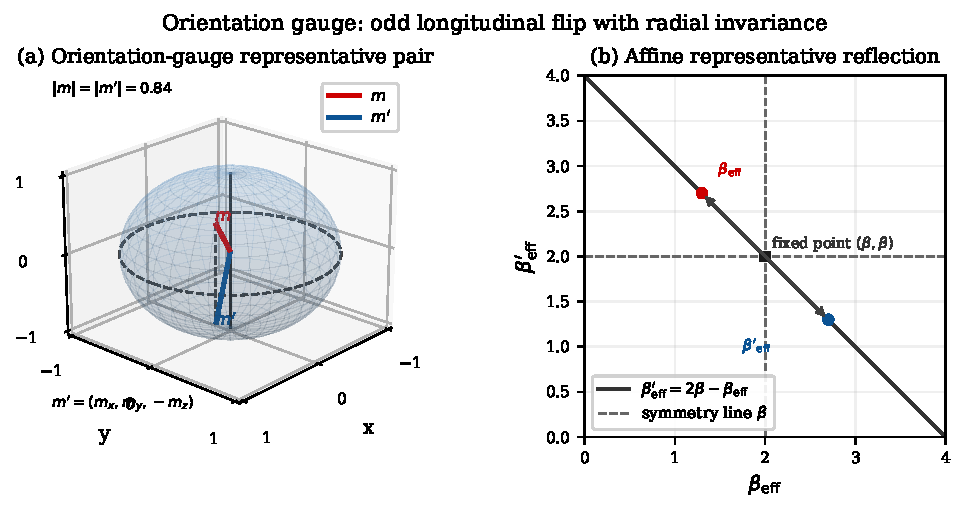
\includegraphics[width=\columnwidth]{../figures/hmf_orientation_gauge_bloch.pdf}
  \caption{
  Geometric action of orientation gauge.
  \textbf{(a)} Bloch-sphere representative pair \(m\) and
  \(m'=(m_x,m_y,-m_z)\): radius is invariant while longitudinal orientation flips.
  \textbf{(b)} Effective-temperature representative reflection
  \(\beta_{\mathrm{eff}}'=2\beta-\beta_{\mathrm{eff}}\), with fixed point
  \((\beta,\beta)\).
  }
  \label{fig:orientation_gauge_bloch}
\end{figure}

\paragraph{Practical consequence.}
When two data points differ only by orientation gauge, radial diagnostics should collapse directly,
while oriented diagnostics should match only after the affine map
\(\beta_{\mathrm{eff}}\leftrightarrow 2\beta-\beta_{\mathrm{eff}}\) is applied.

\paragraph{Formal statement.}
Lemma-level statements and short proofs are collected in
the Appendix.
